

\chapter{The DPI system: Bro} \label{chap:bro}
Bro is an open-source, multi-layered, stream-oriented intrusion detection system capable of high-performance analysis and logging. This section will cover how Bro functions. In particular, we will go over each component's job, how it works, and how they all fit together to provide many flexible services.

\section{System Architecture}
Bro's operation is mainly split into two parts: the C++ Event Engine  and the Policy Script Interpreter. Figure \ref{pic:arch} shows Bro's architecture as seen in the documentation, though it is worth noting that packets can also be fed into the Event Engine through packet captures. \\


\begin{minipage}[c]{\textwidth}
\centering
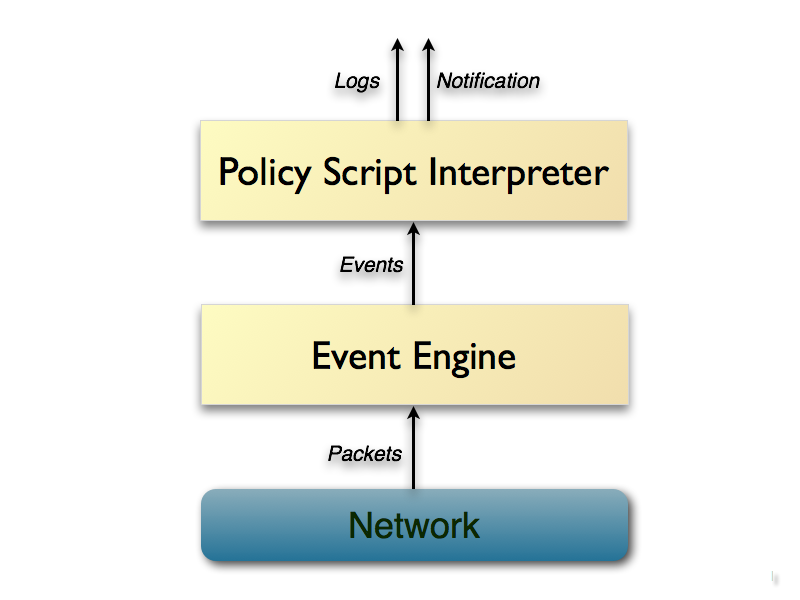
\includegraphics[scale=0.3]{Figures/architecture.png}
\captionof{figure}{Bro's internal architecture}
\label{pic:arch}
\end{minipage} \\

%\begin{figure}[!t]
%\centering
%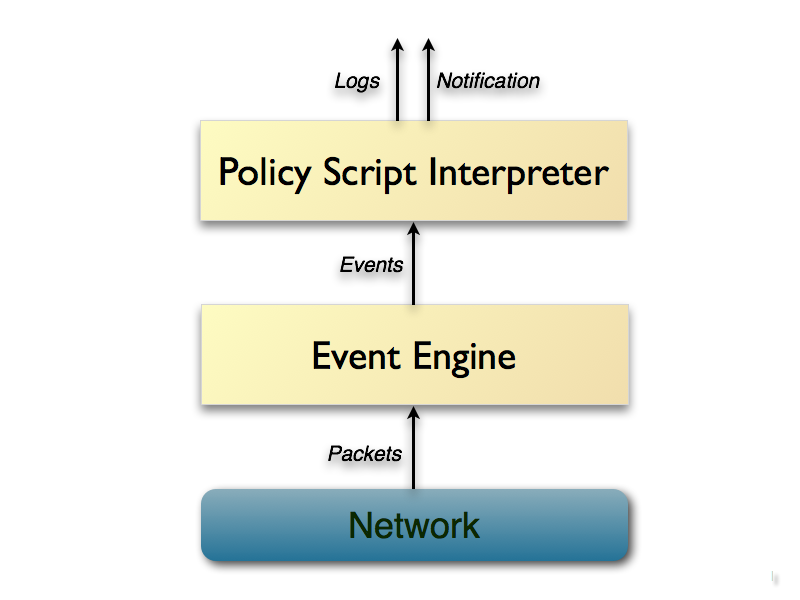
\includegraphics[scale=0.3]{Figures/architecture.png}
%\caption{Bro's internal architecture}
%\label{pic:arch}
%\end{figure}


The Event Engine parses incoming packets and raises events based on what is seen. The engine itself is stream-based and stateful, meaning that it stores information about each stream observed in the network and that packets in a same stream are treated as such. The script interpreter is where events are processed in order to extract meaningful information about the network traffic.\\

The Script Interpreter is the most flexible part of the Bro system. Indeed, Bro ships with a plethora of pre-written scripts that will, for example, log connections for many standard protocols. The great flexibility, however, comes from the fact that anyone can write additional script using Bro's domain specific language (.bro extension). This language is Turing complete, has many pre-defined data structures for network analysis (such as \texttt{addr} which stores both IPv4 and IPv6 addresses or domain names), and allows the users to write their own event handlers to detect the behavior they wish to observe. The script interpreter is also highly stateful, allowing users to store any information they wish to extract from the events that are processed.\\

These two components are not independent, however. Indeed, the Engine is aware of the events, data structures, and even functions that are defined  for scripts (in \texttt{.bif} files). The Engine's event handler is even made aware of which events are actually used in the scripts that are loaded at runtime.

\section{The Event Engine}
As mentioned already, the Event Engine is responsible for parsing packets and generating events. Figure \ref{pic:callstack} shows the stack call for how an event is raised. As we can see, packets are first dispatched to their session, or stream. Once there, the Engine attempts to determine which protocols are in use. This is always done by first determining the transport layer protocol (IPv4 and IPv6 are treated the same way). Once the transport protocol is identified, the packet is sent to the corresponding analyzer through the \texttt{DeliverPacket} method. The figure shows that the packet being processed was found to be using TCP, and was therefore delivered to the \texttt{TCP\_Analyzer}. The analyzer itself contains the logic to analyze the header of the given protocol and raise the corresponding event. Once the analysis is complete, the packet payload is sent to several higher-level analyzers to determine which application layer protocols are used and raise the events concerning those. \\

\begin{figure}[!t]
\centering
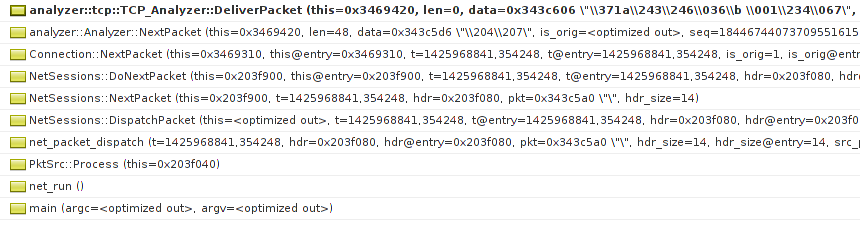
\includegraphics[width = \textwidth]{Figures/brodebug.png}
\caption{Bro call stack to deliver TCP packet}
\label{pic:callstack}
\end{figure}

During the whole process, it is important to remember that all the packets belonging to the same stream are treated together. For some protocols, TCP included, Bro can perform re-assembly internally and deliver the re-assembled stream to the analyzers instead of individual packets. This will play a role on how MPTCP re-assembly must be performed. Indeed, MPTCP must re-assemble content from multiple streams, meaning that the architecture of the Event Engine is not currently adapted to this. It has no way of maintaining state over multiple stream.


\section{The Policy Script Interpreter}
The Script Interpreter manages all the event handlers that are defined in the scripts. Everything that Bro outputs comes from behavior described in one or more scripts. When run out of the box Bro will produce many logs. Even these are the result of scripts that are run by default. When running Bro from the command line, the user may specify additional scripts to be used. All the events that are handled in loaded scripts are sent to the Engine in order for them to be raised when encountered. \\

Scripts use an event-driven language specific to Bro. Once again, the language is Turing complete, meaning that we can actually use this language for any computation we would want to do with another language. Users can store variables which will either be scoped only within the given script, globally available for all scripts running on the machine, or even within a single event handler. Bro's script language features many common data types (such as \texttt{int} and \texttt{count}  which are 64-bit signed and unsigned, respectively, numbers), data structures (such as \texttt{set} for lists of unique elements, \texttt{table} to store key-value pairs...), and custom data types useful for network-related operations (\texttt{addr} for IP addresses, \texttt{port} for port numbers and their associated protocols ...). We can also define our own data structures, called records. \\

Scripts are organized into modules to allow one script to access variables or functions of another by using its name space. For example, calling the \texttt{Log} module's \texttt{create\_stream} function will be done within another script by using \texttt{Log::create\_stream}. The script itself is composed of three main parts. First, an \texttt{export} block defines all the constants that will be used. These include global constants that can be redefined, making the new version of the constant available to all scripts. Examples of this are the Notice and Log entry types which will be discussed in section \ref{output}. New global constants and records are also declared here. Next, users can define functions within their script. This is done as in most any other programming language. The last and most important part is the definition of event handlers. \\

Event handlers are what makes the language event-driven. So far, functions and constants have been defined, but the script doesn't do anything. As in any event-driven language, the script will actually do work when events happen. Even a basic ``hello world'' example is done by writing the traditional print command in an event handler: \\

\begin{code}
event bro_init() {
	print("hello world\n");	
}
\end{code}

An event handler is declared using the \texttt{event} keyword, followed by the type of event that will trigger it (in the hello world example, the event used is \texttt{bro\_init}, which is raised when Bro is started). The arguments of the handler correspond to the data fields of that event. Each time the event is raised, the code of the handler is executed. \texttt{bro\_init} doesn't send any data, but more complex events must always have the same fields as the events defined in the corresponding \texttt{.bif} file. Otherwise, the event is unknown to the system.

\section{Output} \label{output}
Scripts perform the analysis of the network traffic, but once it is done, the results must be output in some form and not stored indefinitely in memory. Rather than having users write their own messages to files, Bro provides two main output methods: logs and notices. Both come with their own framework which allows users to access these high-level functionalities easily.

\subsection{Logging} \label{section: logging}
Bro's logging framework provides a high-performance way to log behavior in standard tab-separated files. Creating a new log file is done entirely in script. The first step is to make the Interpreter aware of the new log by re-defining the \texttt{Log::ID} constant in the scripts \texttt{export} block. This constant contains the IDs of each log currently being maintained, and is populated by default with many common logs such as the connections log. We redefine it using the \texttt{redef} command: \\

\begin{code}
export {
	redef enum Log::ID += { LOG };
	
	
	...
}
\end{code}

Once this is done, we must create a new record (in-script data structure) called \texttt{Info} which will contain the column names for our log. This is also done within the \texttt{export} block. In the record, we specify the name and data type of each column. We are not required to write every element of the record to the log; we must actually specify, for each value, whether or not it must be written to the log with the \texttt{\&log} keyword. Furthermore, we are allowed to have some elements of the record be optional with the \texttt{\&optional} keyword. For example, if we wanted to log an address and port number, we could create a record like so: \\

\begin{code}
	type Info: record {
		address:		addr &log;
		port:			port &log;	
	};
\end{code}

The logging framework manages the logs by creating a stream for each individual log. This stream receives all the entries that are generated for its log and is in charge of writing them to the corresponding file. The next step is therefore to create this stream. To do so, we simply call the \texttt{Log::create\_stream} function. This function takes two arguments: the ID of the log to create, and the record type that will serve as the log header. The call we most often be made within the \texttt{bro\_init} event handler to ensure the stream is up and ready before any entries are generated, and will most often look like this:\\

\begin{code}
	Log::create_stream(LOG, [$columns=Info]);
\end{code}

Now that the stream is created, we simply need to generate its entries when we observe the behavior we are interested in. For example, if we wanted to log the address and port of the originator of every TCP SYN packet we saw, we could write our entry generation in the \texttt{connection\_SYN\_packet} event handler. This would look like: \\

\begin{code}
event connection_SYN_packet(c: connection, pkt: SYN_packet) {
		Log::write(MyModule::LOG, [	$address=c$id$orig_h,
									$port=c$id$orig_p]);
}
\end{code}

Here we see that we fill the fields of the \texttt{Info} record by accessing the fields of the \texttt{connection} record that was sent in the event. The resulting log would resemble:

\begin{code}
#separator \x09
#set_separator	,
#empty_field	(empty)
#unset_field	-
#path	MyModule
#open	2015-05-04-18-57-53
#fields	address	port	
#types	addr	port
2a02:a03f:2214:b200:147:1f2:679d:1ecd	53013
2a02:a03f:2214:b200:147:1f2:679d:1ecd	55243
2a02:a03f:2214:b200:204:4bff:fe0a:54f9	40886
#close	2015-05-04-18-57-54
\end{code}


\subsection{Notices} \label{section: notice}
Logging is important, and parsing logs is a common way to detect that certain attacks took place. However, in many cases we may be interested in a more immediate reaction. This is the Notice framework's purpose. Notices are created in a way very similar to log entries, and they are raised much like log entries are written. Like for Logs, we first begin by redefining the list of known notice types: \\

\begin{code}
	redef enum Notice::Type += { MyNotice, };
\end{code}

This time, we do not define our own \texttt{Info} record because the notice framework uses its own: \texttt{Notice::Info}, defined in \texttt{/scripts/base/frameworks/notice/main.bro}. A quick inspection of the record shows that it provides many fields to transmit information to the function that will handle the notice. Most of these fields, however, are optional, and we therefore need only send the information of interest for a given event.\\

The next step is actually raising the notice. This is done in a similar way as creating a log entry, only simpler. Indeed, we only need to call the \texttt{NOTICE} function which takes a \texttt{Notice::Info} record as argument. Returning to our earlier example of TCP SYN packets, we could raise a notice for every one instead or in addition to logging it. This would be done as follows:

\begin{code}
event connection_SYN_packet(c: connection, pkt: SYN_packet) {
		NOTICE([$note=MyNote,
                $msg=fmt("SYN received from %s", c$id$orig_h)]);
}
\end{code}

Once again, most fields of the \texttt{Notice::Info} record are optional. Here, we filled \texttt{note} which is the notice type which allows the notice handler to distinguish which kind of notice it was (and the only mandatory field), and \texttt{msg} which allows us to transmit a human-readable message along with the notice.\\

Once the notice is raised, it will not be acted upon unless a script subscribes notices by using a hook. The hook will be executed every time a notice is raised, and can check the note to determine which notice took place, and how to react to it. For our example, we could write a hook that sends an e-mail every time the notice is raised (a very bad idea in practice, of course): \\

\begin{code}
hook Notice::policy(n: Notice::Info) {
    if (n$note == MyModule::MyNoticer) {
        add n$actions[Notice::ACTION_EMAIL];
    }
}
\end{code}

